

\documentclass[12pt, a4paper]{article}


\usepackage{fancyhdr, enumerate}
\usepackage{amssymb}
\usepackage{geometry, amsmath, amsfonts, float, graphicx}
\usepackage{gensymb}
\usepackage{hyperref, listings}
\usepackage{matlab-prettifier}
\usepackage{caption}
\geometry{
	top=0.9in,           
	inner=0.6in,
	outer=0.6in,
	bottom=2in,
	tmargin= 10ex,       
	headsep=0.6cm,          
}
\pagestyle{fancy}

\fancyhead{}
\fancyfoot{}

\fancyhead[L]{Bioen 316 AC \\Homework 2\\ April 10, 2019}
\fancyhead[R]{Skyler Hallinan\\ hallisky@uw.edu \\ 1732227}

\lstMakeShortInline[style=Matlab-editor]"
\begin{document}
\vspace*{-3mm}
\section*{Problem}
Suppose that you are using a 16-bit analog-to-digital converter (ADC) as part of an
electroencephalograph, and that you have set up the ADC to capture signals over the range
[–10 V, +10 V]
\begin{enumerate} \item
 \begin{enumerate} \item
What is the voltage resolution of the ADC?
\item
Suppose that the least significant bit (LSB) stops working (is always 0) but the other 15
bits are OK. How does this fault affect the values that the ADC sends to the computer as it
samples the voltage measured on the scalp? Specifically, what is its effect on the voltage
range and resolution of the system?

\item
If the most significant bit (MSB) stops working (is always 0) but the other 15 are OK,
what is the effect on the voltage range and resolution of the system?

\item
If only the 14th bit fails (i.e. the bit two to the right of the most significant bit), could you
still use the ADC? What limitations would you need to place on the input range(s)? Explain
your answer, including a figure that plots apparent voltage (the voltage value that the ADC
sends to the computer) vs. the actual voltage that is input to the ADC.
 \end{enumerate}
 \end{enumerate}
\section*{Solution}


\begin{enumerate}
\item
\begin{enumerate}
\item  
 We can use the following formula to determine the smallest measurable volage increment represented by the least significant bit: $ q \approx \frac{\Delta V}{2^b}$, where $\Delta V = V_{in, max} - V_{in, min}$, $b$ is the number of bits, and $q$ is the smallest measured voltage increment, otherwise known as the voltage resolution. We see that $\Delta V = (16 - (-16)) \times 10^{-3} = 32 \times 10^{-3}$, $b = 16$, and $q = 5\times 10^{-7}$. \\ \\
We see that the input voltage is $\pm 10 $ V, which correponds to an input voltage range of 20; $\Delta V = (10 - (-10)) = 20$. In addition, we see that our our ADC converter uses 16 bits; $b = 16$. Therefore our only unknown component is our voltage resolution. \\ \\
Using the above values, we see that we can calculate the voltage resolution as follows: 
\begin{align*}
 q &\approx \frac{\Delta V}{2^b} \\
 &= \frac{20}{2^{16}} \\
&= \frac{5}{16384} \\
&\approx 3.05 \times 10^{-4}
\end{align*}
Therefore our voltage resolution is $\frac{5}{16384}$ or $3.05 \times 10^{-4}$ V.
%
%\begin{figure}[h]
%\centering
%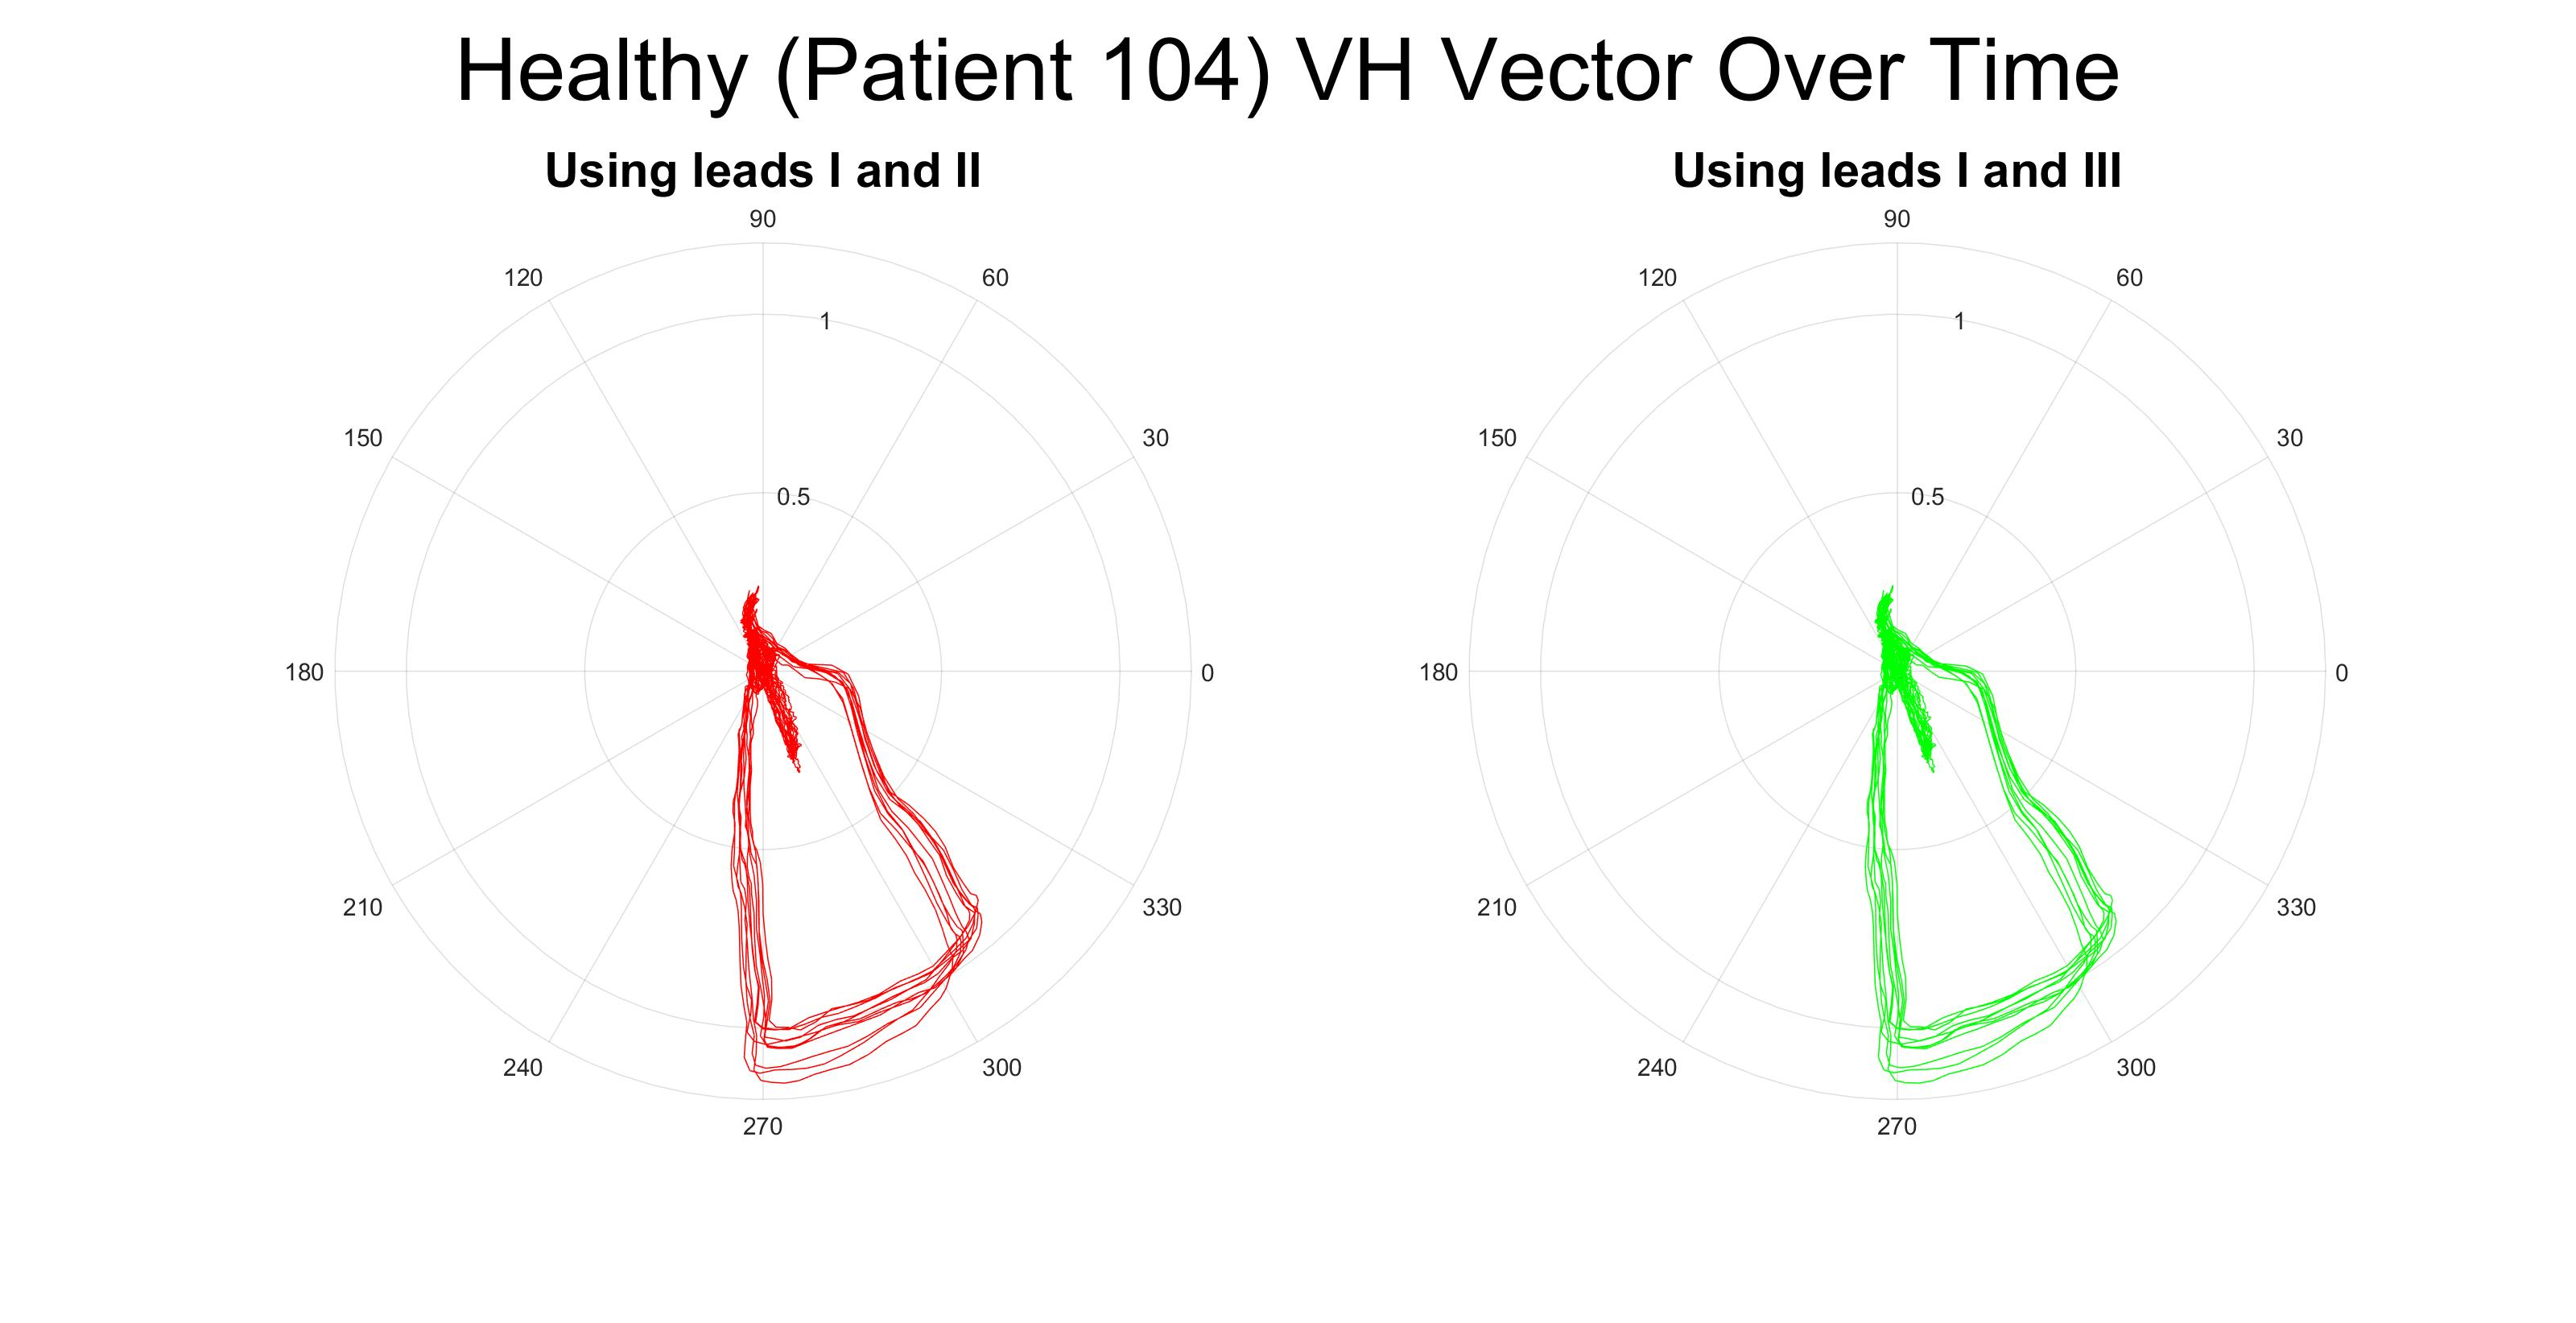
\includegraphics[width=1\textwidth]{ecg1}
%\caption{Healthy Patient Heart Vector Derived from Leads I and II (left) and I and III (right)}
%\end{figure}


\item 
If our least significant bit stops working, then we will only have a 0 at our bit corresponding to $2^{0}$. In our ADC converter, a single bit corresponds to the voltage resolution increase that we calculated before; one bit in the 16 bit system should correspond to a voltage ``bin'' of $3.05 \times 10^{-4}$ V. Our least significant bit represents the smallest detectable voltage increment, and is the minimum voltage difference that can be normally captured by two different 16-bit encodings normally. If, however, our least significant bit does not work, we will not be able to differentiate between two voltages $3.05 \times 10^{-4}$ V apart; normally these would be separately represented by a 1 bit difference (on the least significant bit). Now, however, since the least significant bit is always 0, our ADC converter will interpret, for example, voltages 0 and $3.05 \times 10^{-4}$ V the same, as the binary encoding for them will now be the same. So, in our ADC converter, these two voltages, which would normally be stored as different encodings in a working system, will now be considered the same; our resolution interval size increases. \\ \\
In our new system, since our least significant bit no longer works, we have to rely on the $2^{1}$ bit to differentiate between different voltages. We go from an old voltage resolution of $q * 2^0 = 3.05 \times 10^{-4}$ to a new voltage resolution of $q * 2^{1} = 6.10 \times 10^{-4}$; we basically can only count by 2s now with the $2^1$ bit, and cannot use the $2^0$ bit to increment in sizes of our original $q$ anymore. Our new voltage resolution is twice of our original one. This makes sense; we are basically removing half of the data that we can represent, which is reflected by the doubling of voltage resolution size. \\ \\
Our voltage range represented will be largely unchanged; the voltage resolution will only affect the small ``bins'' by which different voltages are differentiated; there are half of them now, but they are double the size. Our lowest voltage is still at -10, while our max voltage that we can accurately detect is approximately 10 as well: Our range is still $\approx$ [-10, 10] V. (Our maximum accurately detectable voltage is technically 10 - ($3.05 \times 10^{-4}$ )because we removed the upper end differentiation that lets our ADC converter tell the difference between 10 - ($3.05 \times 10^{-4}$) and 10 via the 16 bit system; an input voltage of 10 will now be incorrectly stored by the ADC in 16 bit as a voltage of 10 - ($3.05 \times 10^{-4}$)). 
In conclusion, removing the least significant bit does not affect the voltage range at which we can represent our voltages, but it does increase the voltage resolution size by a factor of 2, since our least significant bit cannot be expressed.

\item
If our most significant bit is not represented, then out of the $2^{16}$ possibilities in a 16 bit system, we can only represent up to the first $2^{15}$ of them. That is, with a maximum value of our 16 bit system ranging from values from 0 to $2^{16} - 1$, since we only can use 15 bits, our highest value we can get results in a range from 0 to $2^{15} -1$.  This means that we can effectively only capture the first half of the voltage range.\\ \\
We multiply this highest bit value by our voltage resolution $q$ to get a sense of what voltages we can capture with these constraints. We see that $Max = (2^{15} - 1) \cdot 3.05 \times 10^{-4} = 9.9969 \approx 10$. Therefore, from our total voltage range initially of 20 V, we can now only capture the first 10 V accurately, that is, only [-10,0] can accurately be represented by the ADC converter. \\ \\
For voltages above this limit, they require the 16th bit to be represented. In this case, when going from input signal to ADC converter signal, there would normally be a 1 value in this 16th bit. However, when these values now go into the ADC converter, they are represented as 0; therefore, these voltages are missing a $2^{15}$ component (that is the value represented by the 16th bit), which corresponds to a $2^{15} \cdot q \Rightarrow 2^{15} \cdot 3.05 \times 10^{-4} = 10$ V loss; values above 0 V in our system (from 0 to 10 V) are actually represented as -10 to 0 by our ADC converter, and are therefore incorrectly labeled. \\ \\
In conclusion, we see that removing our most significant bit decreases our accurate ADC conversion range from [-10,10] V to [-10,0] V. At values above 0 V in our system, our ADC converter misclassifies their voltage as 10 less than what they actually are. However, our voltage resolution is still the same.
\item 
If only the 14th bit fails, there will be slightly more complicated calculations needed. Essentially, we will have to look at the possible values captured when our 15th and 16th bit combinations are 00, 01, 11, and 10. Here is our logic: \\ \\
If the 14th bit fails, we can still store the first $2^{13}$ bits successfully, with a value range from 0 to $2^{13} - 1$; this corresponds to the first 13 bits having a value of 1. \\ \\ 
Then, because we do not have a 14th bit, the next highest number we can store would correspond to a 1 in the 15th bit location, with a 0 everywhere else. This corresponds to a value of $2^{14}$, as the 15th bit is the $2^{14}$ slot. Then, using the same logic as the previous part, the highest value with this 15th bit 1 and the 16th bit 0 we could achieve would be when now when the first 13 bits are also 1, which gives us a value of $2^{14} + 2^{13} - 1$ (upper range limit). Thus, our range we could represent here is $2^{14}$ to $2^{14} + 2^{13} - 1$. \\ \\
Now, we have another gap, as we cannot fill in the 14th bit. The next highest number we can store successfully corresponds to when only the 16th bit is 1, and every other bit is 0. This results in a value of $2^15$ (value of 16th bit). The endpoint to this range, similarly to when we just had the 15th bit filled, is just $2^{15}$ + $ 2^{13} - 1 $, where the  $2^{13} - 1$ still corresponds to the max value of the first 13 bits. Therefore we have a range from $2^{15}$ to $2^{15}$ + $ 2^{13} - 1 $. \\ \\
Finally, we have our last gap. Our next highest number we can represent is when only bits 16 and 15 are filled. This corresponds to a value of $2^{15} + 2^{14}$. Once again, we add the highest value of the first 13 bits, $ 2^{13} - 1 $, to this starting point to determine our range. We get a range of  $2^{15} + 2^{14}$ to $2^{15} + 2^{14} + 2^{13} - 1$ that can be represented.  \\ \\
In total, we have the ranges that can be represented correctly as following: \begin{align*}
Range = \{ [0, 2^{13} - 1], [ 2^{14} ,2^{14} + 2^{13} - 1], [2^{15},2^{15} +  2^{13} - 1], [2^{15} + 2^{14}, 2^{15} + 2^{14} + 2^{13} - 1]\}
\end{align*}
We multiply by our voltage resolution $q \approx 3.05 \times 10^{-4}$ to convert these to our scale of 20 volts, and get:
\begin{align*}
Range = \{ [0, 2.49969], [ 5 , 7.49969], [10, 12.49997], [15, 17.4997]\}
\end{align*}
Finally, we shift these down by 10 to see what our practical range we can cover accurately is:
\begin{align*}
Range = \{ [-10, -7.5], [-5 , -2.5], [0, 2.5], [5, 7.5]\}
\end{align*}
Thus, for voltage values in these small ranges, our ADC converter will properly convert our signal, as these are not affected by the 14th bit. \\ \\ What happens at values in between the interval though? At locations where there would normally be a 14th bit represented (by a 1), which happens at locations in the interval between [-10,10] V \textbf{excluded} in this $range$, there is none. Therefore, we need to subtract the 14th bit value from all these locations, to find out what the ADC converter would represent these numbers as (inaccurately). We see that this 14th bit value corresponds to $2^{13} * q \Rightarrow 2^{13} * 3.05 \times 10^{-4} = 2.5$. Therefore for those values not in the $range$, they will be represented by the ADC converter inaccurately as 2.5 less than their actual value. In our entire system, the voltage resolution is unchanged.

\begin{minipage}[t]{\linewidth}
\centering
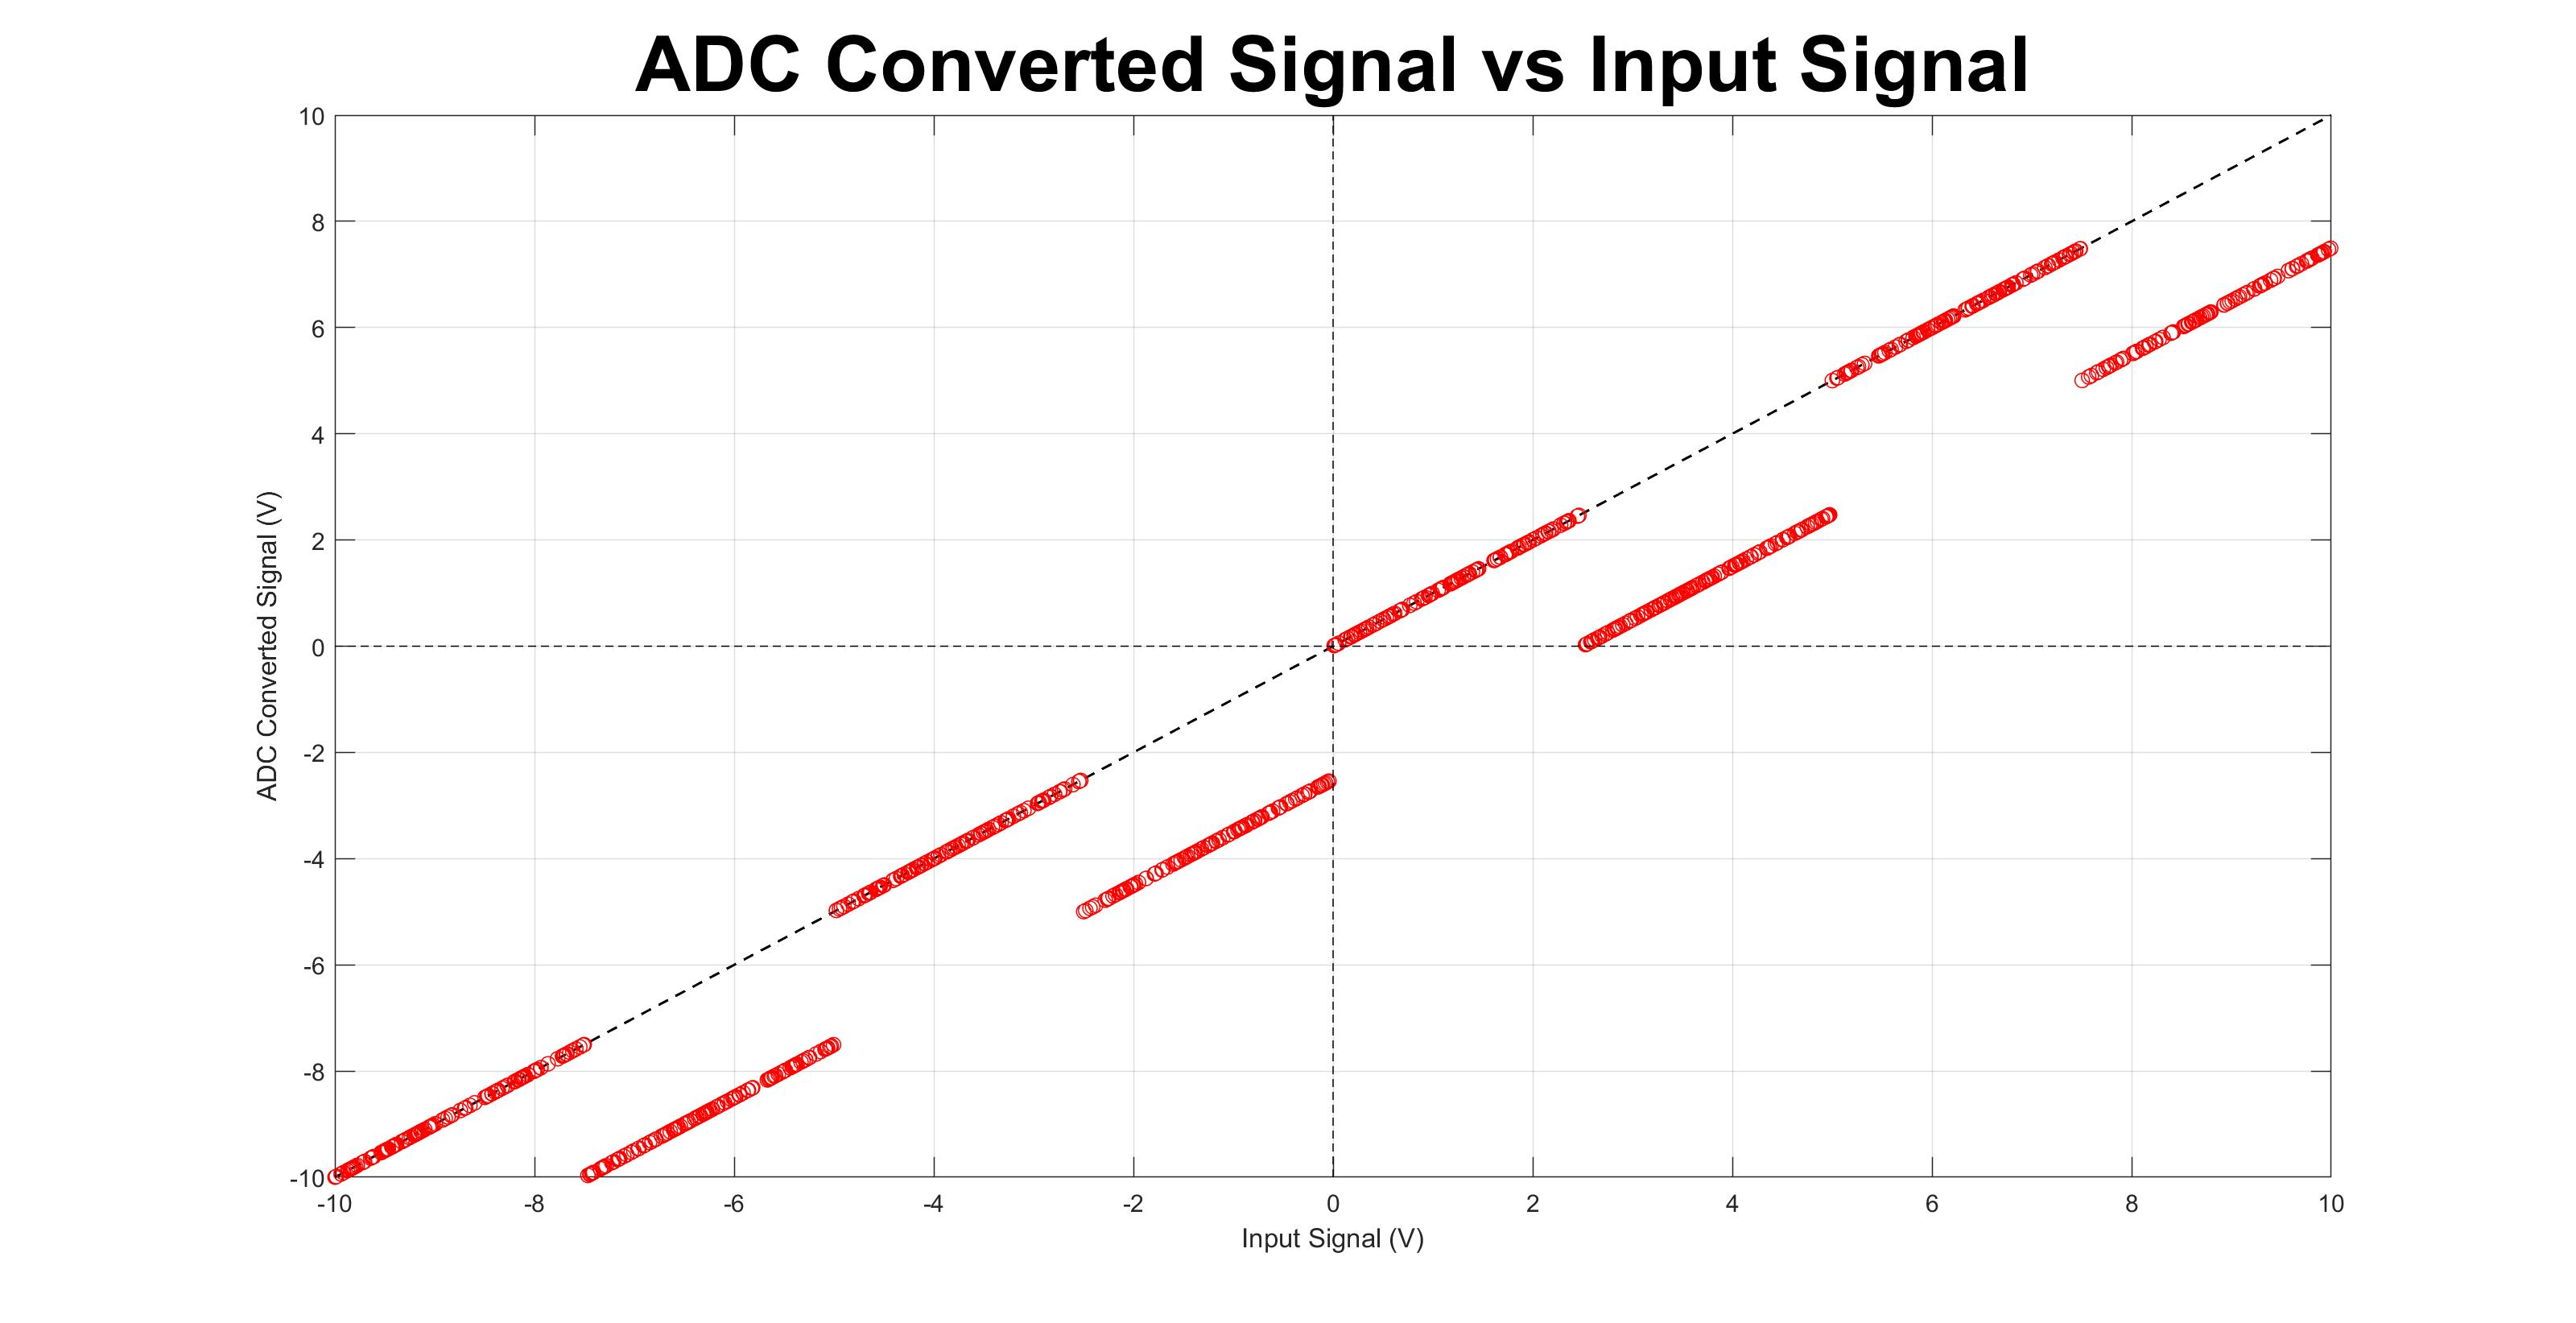
\includegraphics[width=1\textwidth]{hw22}
\captionof{figure}{ADC signal vs an input signal (1000 points)}
\end{minipage} \\ \\
\end{enumerate}

We generated 1000 points of random data between [-10,10] and plotted what the converted signal would look like compared to the input signal. We see that our graph of ADC Converted Signal vs Input Signal represents this. In the range $Range = \{ [-10, -7.5], [-5 , -2.5], [0, 2.5], [5, 7.5]\}$, the graph follows the line $y= x$; that is, the ADC converted signal and the input signal match up. However, outside this range, the values are shifted down by a value of 2.5 from this line. This creates a discontinuous curve, and matches our calculations from above.

\begin{minipage}[t]{\linewidth}
\centering
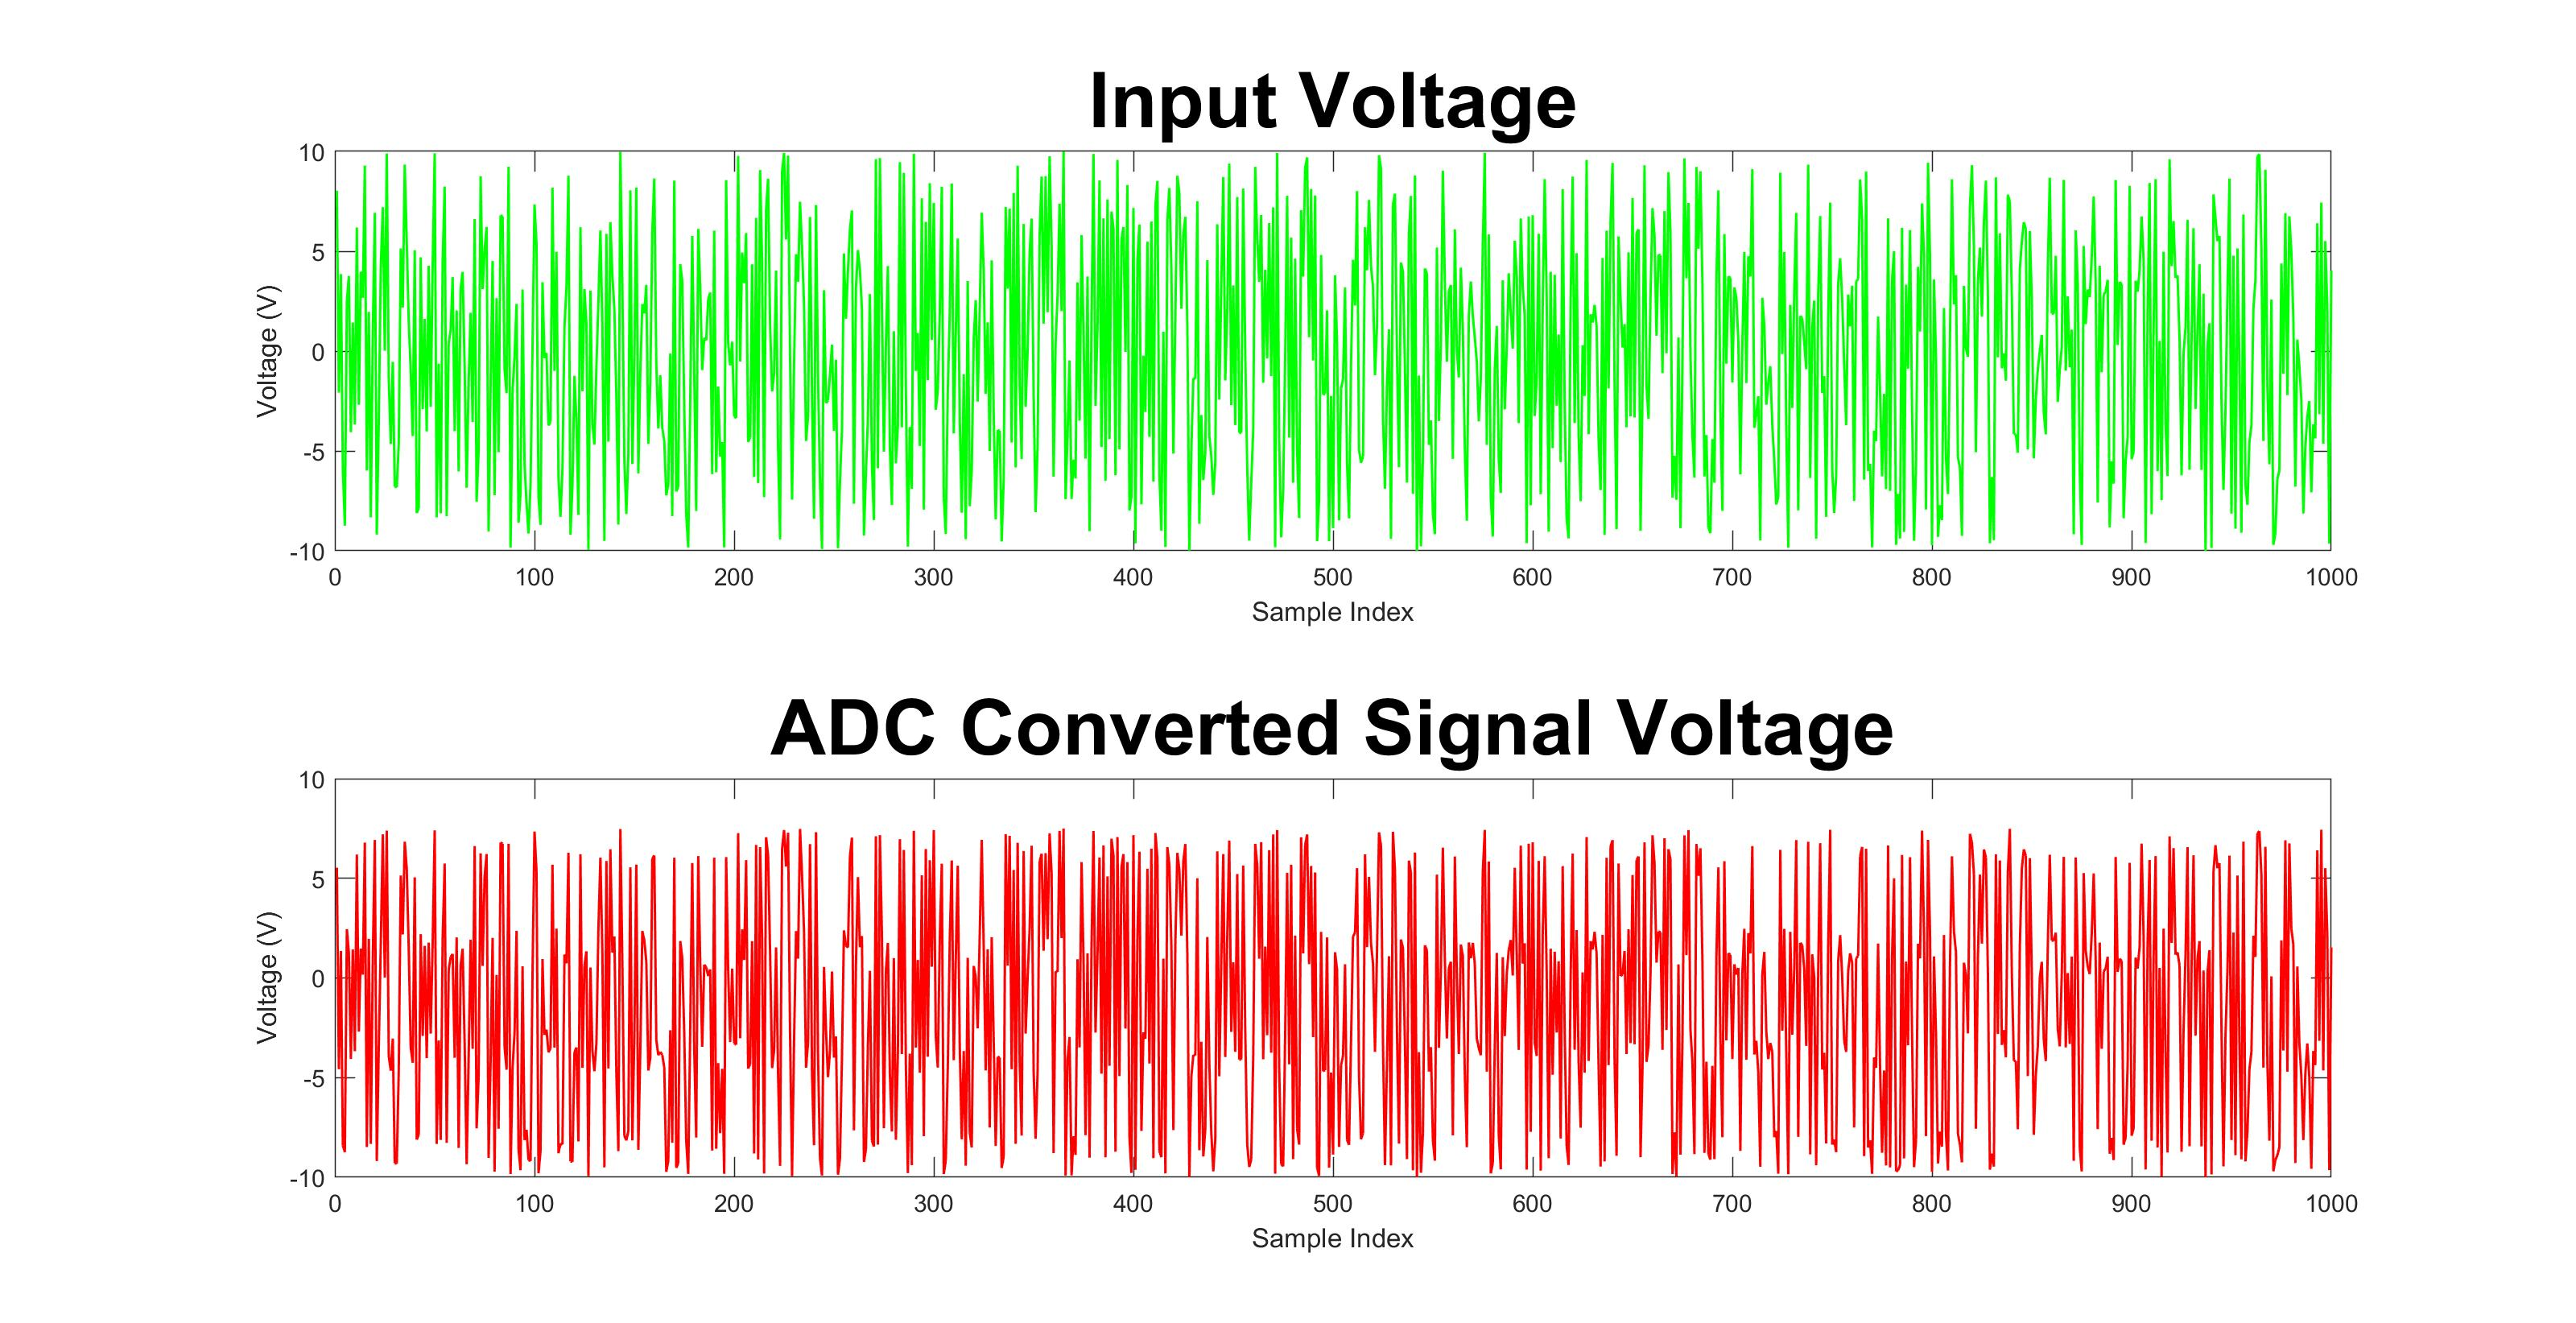
\includegraphics[width=1\textwidth]{hw21}
\captionof{figure}{ADC signal and input signal vs index of signal}
\end{minipage} \\ \\ \\
We see that time-series representation of this random 1000 index data looks like the representation in Figure 2. We see clearly that ADC is unable to cover the high end ranges (7.5 - 10), as well as others, which we clearly calculated. Our sample index can be also viewed as a time component, but this dataset was arbitrarily created.

%still can have first 2^13
%max value (11111 for 13 bits) is 2^13 -1
%skip 14th bit
%min value with 15th bit representation is just 2^14 (15th bit is the 2^14 slot)
%
%can represent from 0 to 2^13 - 1 then a gap
%then goes to 2^14 to 2^14 + (2^13 - 1)
%
%another gap: min value for the 16th bit is 2^15
%can go from 2^15 to 2^15 + (2^13 -1) (we have a 0 value 15th bit here)
%next interval is 2^15 + 2^14 to 2^15 + 2^14 + 2^13 -1 (we have a 1 value 15th bit here) 

\end{enumerate}
\pagebreak
\section*{\fontsize{19}{15}\selectfont Appendix A}
\subsection*{MATLAB code}
\lstinputlisting[style=Matlab-editor]{hw2.m}
\end{document}